% !TEX encoding = UTF-8
% !TEX TS-program = pdflatex
% !TEX root = ../tesi.tex

%**************************************************************
\section{Kitti}
\label{sec:kitti}
%**************************************************************

The odometry benchmark consists of 22 stereo sequences, saved in loss\-less png format: 11 sequences are provided with ground truth trajectories for training (0-10) and 11 sequences (11-21) without ground truth trajectories for evaluation.

This odometry benchmark is a subset of KITTI Vision Benchmark suite by Geiger et al.~(\cite{kitti_dataset}).

\subsection{Scene}\label{subsec:kitti-scene}
The images represent a various of scenes from mid-sized city, rural areas and on highways.
\begin{figure}[H]
    \centering
    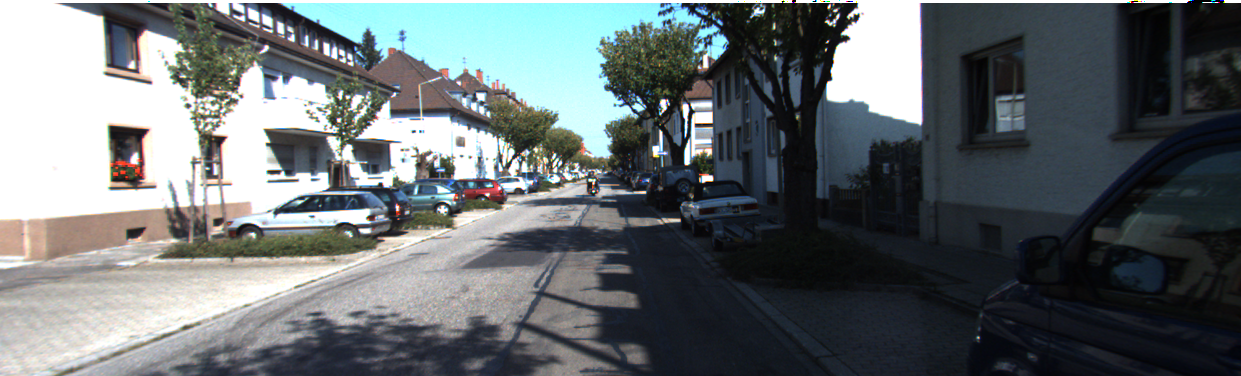
\includegraphics[width=\textwidth]{images/3_1_example_kitti_scene}
    \caption{KITTI - example of scene}\label{fig:example-of-kitti-scene}
\end{figure}

\subsection{Image generation}\label{subsec:kitti-image-generation}
Each sequence of the KITTI dataset is composed of by four sequences of images: left-coloured, right-coloured, left-grey and right-grey.
Each one is captured by a camera mounted on the top of vehicle.
They calibrated the four video cameras intrinsically and extrinsically and rectified the input image.
Then they computed the 3D rigid motion parameters which relate the coordinate system of the laser scanner.

Meanwhile, the ground-truth is directly given by the output of the GPS/IMU localization unit projected into the coordinate system of the left camera after rectification.

\subsection{Dataset statistics}\label{subsec:kitti-dataset-statistics}
The dataset consists of 22 stereo sequences, with a total length of 39.2 km, which was the longest in the time of the publication of the paper.
In the dataset, there are no specifically indicate which sequence is used for training, validation or testing, but in this work, the dataset is split as this:
\begin{table}[H]
    \centering
    \begin{tabular}{|c|c|c|}
        \hline
        \textbf{Sets}           & \textbf{N. of Sequence} & \textbf{N. Image} \\ \hline
        \textbf{Training set}   & 8                       & 20.098            \\ \hline
        \textbf{Validation set} & 2                       & 1.902             \\ \hline
        \textbf{Test set}       & 1                       & 1.201             \\ \hline
        \textit{\textbf{Total}} & 11                      & 23.201            \\ \hline
    \end{tabular}\caption{KITTI - dataset statistics}\label{tab:kitti-dataset-statistics}
\end{table}

The images dimensions about 1240x370 are slightly different, generally varying for few pixels.
\subsection{Usage}\label{subsec:kitti-usage}

This dataset is the one mainly used, as it is the one of the most famous and most used in the literature.

The sequence \textbf{3} and \textbf{7} are used for evaluation and testing, because they are the easier ones.
\begin{figure}[H]
    \centering
    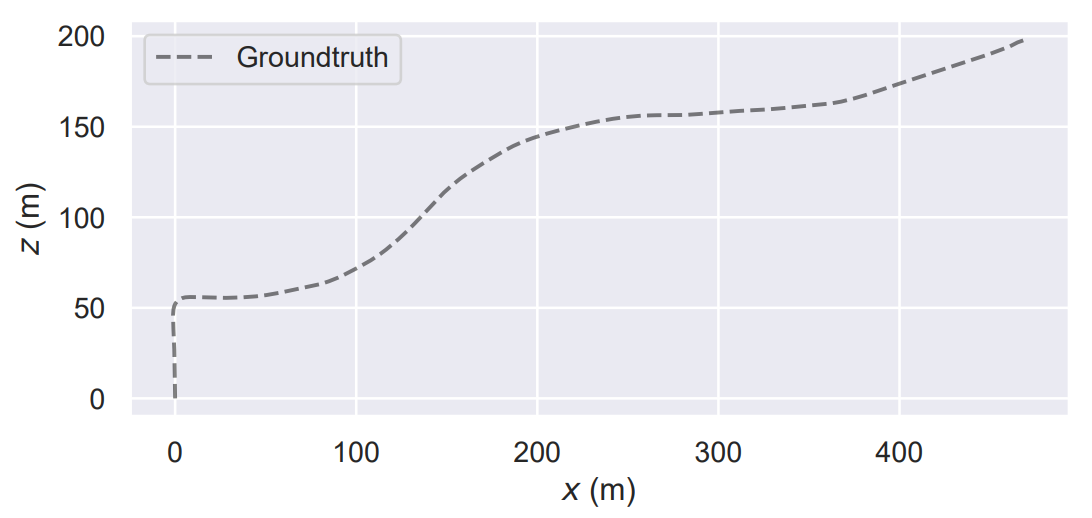
\includegraphics[width=0.5\textwidth]{images/3_1_kitti_seq_3}
    \caption{KITTI - sequence 3}\label{fig:kitti-seq-3}
\end{figure}
\begin{figure}[H]
    \centering
    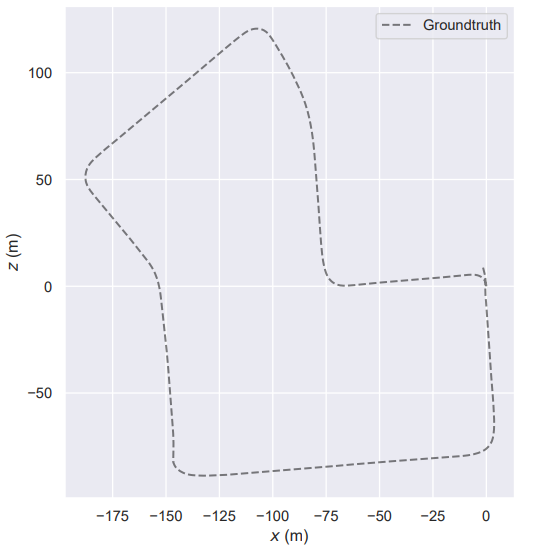
\includegraphics[width=0.5\textwidth]{images/3_1_kitti_seq_7}
    \caption{KITTI - sequence 7}\label{fig:kitti-seq-7}
\end{figure}

Initially, to test the model's capacity, the model was trained and evaluated on the same sequence, to see if it's able to reproduce the ground truth.
Then, the model was fed with more complex sequences.